\documentclass[1p]{elsarticle_modified}
%\bibliographystyle{elsarticle-num}

%\usepackage[colorlinks]{hyperref}
%\usepackage{abbrmath_seonhwa} %\Abb, \Ascr, \Acal ,\Abf, \Afrak
\usepackage{amsfonts}
\usepackage{amssymb}
\usepackage{amsmath}
\usepackage{amsthm}
\usepackage{scalefnt}
\usepackage{amsbsy}
\usepackage{kotex}
\usepackage{caption}
\usepackage{subfig}
\usepackage{color}
\usepackage{graphicx}
\usepackage{xcolor} %% white, black, red, green, blue, cyan, magenta, yellow
\usepackage{float}
\usepackage{setspace}
\usepackage{hyperref}

\usepackage{tikz}
\usetikzlibrary{arrows}

\usepackage{multirow}
\usepackage{array} % fixed length table
\usepackage{hhline}

%%%%%%%%%%%%%%%%%%%%%
\makeatletter
\renewcommand*\env@matrix[1][\arraystretch]{%
	\edef\arraystretch{#1}%
	\hskip -\arraycolsep
	\let\@ifnextchar\new@ifnextchar
	\array{*\c@MaxMatrixCols c}}
\makeatother %https://tex.stackexchange.com/questions/14071/how-can-i-increase-the-line-spacing-in-a-matrix
%%%%%%%%%%%%%%%

\usepackage[normalem]{ulem}

\newcommand{\msout}[1]{\ifmmode\text{\sout{\ensuremath{#1}}}\else\sout{#1}\fi}
%SOURCE: \msout is \stkout macro in https://tex.stackexchange.com/questions/20609/strikeout-in-math-mode

\newcommand{\cancel}[1]{
	\ifmmode
	{\color{red}\msout{#1}}
	\else
	{\color{red}\sout{#1}}
	\fi
}

\newcommand{\add}[1]{
	{\color{blue}\uwave{#1}}
}

\newcommand{\replace}[2]{
	\ifmmode
	{\color{red}\msout{#1}}{\color{blue}\uwave{#2}}
	\else
	{\color{red}\sout{#1}}{\color{blue}\uwave{#2}}
	\fi
}

\newcommand{\Sol}{\mathcal{S}} %segment
\newcommand{\D}{D} %diagram
\newcommand{\A}{\mathcal{A}} %arc


%%%%%%%%%%%%%%%%%%%%%%%%%%%%%5 test

\def\sl{\operatorname{\textup{SL}}(2,\Cbb)}
\def\psl{\operatorname{\textup{PSL}}(2,\Cbb)}
\def\quan{\mkern 1mu \triangleright \mkern 1mu}

\theoremstyle{definition}
\newtheorem{thm}{Theorem}[section]
\newtheorem{prop}[thm]{Proposition}
\newtheorem{lem}[thm]{Lemma}
\newtheorem{ques}[thm]{Question}
\newtheorem{cor}[thm]{Corollary}
\newtheorem{defn}[thm]{Definition}
\newtheorem{exam}[thm]{Example}
\newtheorem{rmk}[thm]{Remark}
\newtheorem{alg}[thm]{Algorithm}

\newcommand{\I}{\sqrt{-1}}
\begin{document}

%\begin{frontmatter}
%
%\title{Boundary parabolic representations of knots up to 8 crossings}
%
%%% Group authors per affiliation:
%\author{Yunhi Cho} 
%\address{Department of Mathematics, University of Seoul, Seoul, Korea}
%\ead{yhcho@uos.ac.kr}
%
%
%\author{Seonhwa Kim} %\fnref{s_kim}}
%\address{Center for Geometry and Physics, Institute for Basic Science, Pohang, 37673, Korea}
%\ead{ryeona17@ibs.re.kr}
%
%\author{Hyuk Kim}
%\address{Department of Mathematical Sciences, Seoul National University, Seoul 08826, Korea}
%\ead{hyukkim@snu.ac.kr}
%
%\author{Seokbeom Yoon}
%\address{Department of Mathematical Sciences, Seoul National University, Seoul, 08826,  Korea}
%\ead{sbyoon15@snu.ac.kr}
%
%\begin{abstract}
%We find all boundary parabolic representation of knots up to 8 crossings.
%
%\end{abstract}
%\begin{keyword}
%    \MSC[2010] 57M25 
%\end{keyword}
%
%\end{frontmatter}

%\linenumbers
%\tableofcontents
%
\newcommand\colored[1]{\textcolor{white}{\rule[-0.35ex]{0.8em}{1.4ex}}\kern-0.8em\color{red} #1}%
%\newcommand\colored[1]{\textcolor{white}{ #1}\kern-2.17ex	\textcolor{white}{ #1}\kern-1.81ex	\textcolor{white}{ #1}\kern-2.15ex\color{red}#1	}

{\Large $\underline{12n_{0542}~(K12n_{0542})}$}

\setlength{\tabcolsep}{10pt}
\renewcommand{\arraystretch}{1.6}
\vspace{1cm}\begin{tabular}{m{100pt}>{\centering\arraybackslash}m{274pt}}
\multirow{5}{120pt}{
	\centering
	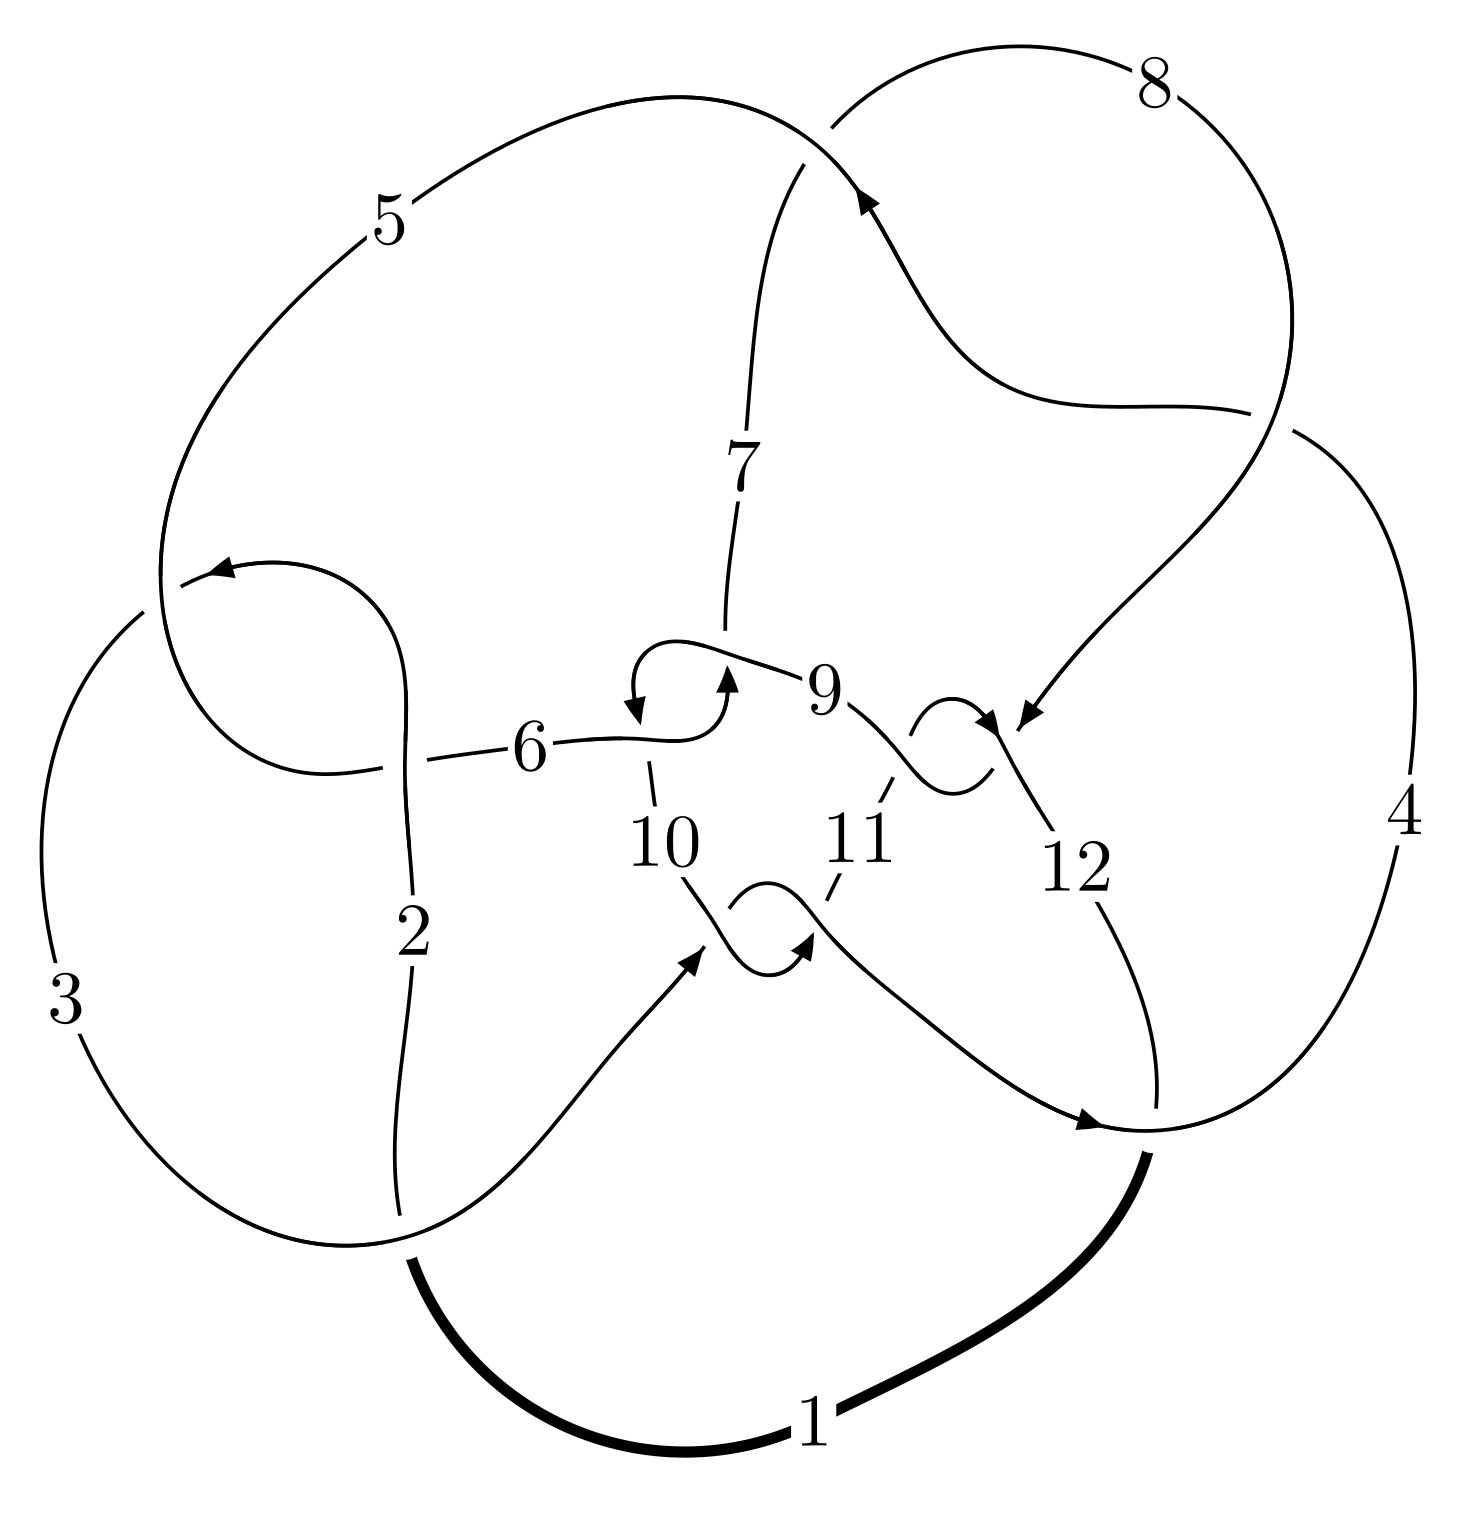
\includegraphics[width=112pt]{../../../GIT/diagram.site/Diagrams/png/2631_12n_0542.png}\\
\ \ \ A knot diagram\footnotemark}&
\allowdisplaybreaks
\textbf{Linearized knot diagam} \\
\cline{2-2}
 &
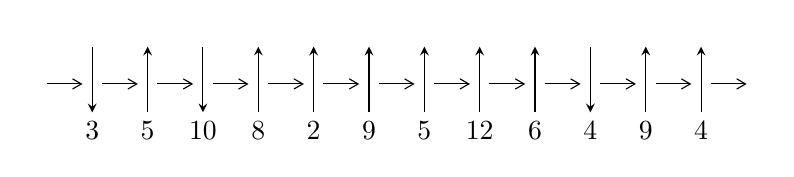
\begin{tikzpicture}[x=20pt, y=17pt]
	% nodes
	\node (C0) at (0, 0) {};
	\node (C1) at (1, 0) {};
	\node (C1U) at (1, +1) {};
	\node (C1D) at (1, -1) {3};

	\node (C2) at (2, 0) {};
	\node (C2U) at (2, +1) {};
	\node (C2D) at (2, -1) {5};

	\node (C3) at (3, 0) {};
	\node (C3U) at (3, +1) {};
	\node (C3D) at (3, -1) {10};

	\node (C4) at (4, 0) {};
	\node (C4U) at (4, +1) {};
	\node (C4D) at (4, -1) {8};

	\node (C5) at (5, 0) {};
	\node (C5U) at (5, +1) {};
	\node (C5D) at (5, -1) {2};

	\node (C6) at (6, 0) {};
	\node (C6U) at (6, +1) {};
	\node (C6D) at (6, -1) {9};

	\node (C7) at (7, 0) {};
	\node (C7U) at (7, +1) {};
	\node (C7D) at (7, -1) {5};

	\node (C8) at (8, 0) {};
	\node (C8U) at (8, +1) {};
	\node (C8D) at (8, -1) {12};

	\node (C9) at (9, 0) {};
	\node (C9U) at (9, +1) {};
	\node (C9D) at (9, -1) {6};

	\node (C10) at (10, 0) {};
	\node (C10U) at (10, +1) {};
	\node (C10D) at (10, -1) {4};

	\node (C11) at (11, 0) {};
	\node (C11U) at (11, +1) {};
	\node (C11D) at (11, -1) {9};

	\node (C12) at (12, 0) {};
	\node (C12U) at (12, +1) {};
	\node (C12D) at (12, -1) {4};
	\node (C13) at (13, 0) {};

	% arrows
	\draw[->,>={angle 60}]
	(C0) edge (C1) (C1) edge (C2) (C2) edge (C3) (C3) edge (C4) (C4) edge (C5) (C5) edge (C6) (C6) edge (C7) (C7) edge (C8) (C8) edge (C9) (C9) edge (C10) (C10) edge (C11) (C11) edge (C12) (C12) edge (C13) ;	\draw[->,>=stealth]
	(C1U) edge (C1D) (C2D) edge (C2U) (C3U) edge (C3D) (C4D) edge (C4U) (C5D) edge (C5U) (C6D) edge (C6U) (C7D) edge (C7U) (C8D) edge (C8U) (C9D) edge (C9U) (C10U) edge (C10D) (C11D) edge (C11U) (C12D) edge (C12U) ;
	\end{tikzpicture} \\
\hhline{~~} \\& 
\textbf{Solving Sequence} \\ \cline{2-2} 
 &
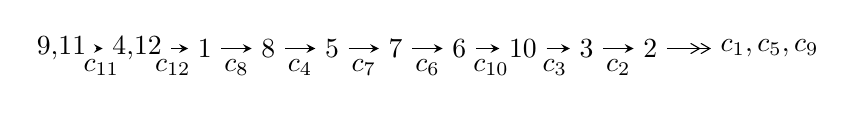
\begin{tikzpicture}[x=23pt, y=7pt]
	% node
	\node (A0) at (-1/8, 0) {9,11};
	\node (A1) at (17/16, 0) {4,12};
	\node (A2) at (17/8, 0) {1};
	\node (A3) at (25/8, 0) {8};
	\node (A4) at (33/8, 0) {5};
	\node (A5) at (41/8, 0) {7};
	\node (A6) at (49/8, 0) {6};
	\node (A7) at (57/8, 0) {10};
	\node (A8) at (65/8, 0) {3};
	\node (A9) at (73/8, 0) {2};
	\node (C1) at (1/2, -1) {$c_{11}$};
	\node (C2) at (13/8, -1) {$c_{12}$};
	\node (C3) at (21/8, -1) {$c_{8}$};
	\node (C4) at (29/8, -1) {$c_{4}$};
	\node (C5) at (37/8, -1) {$c_{7}$};
	\node (C6) at (45/8, -1) {$c_{6}$};
	\node (C7) at (53/8, -1) {$c_{10}$};
	\node (C8) at (61/8, -1) {$c_{3}$};
	\node (C9) at (69/8, -1) {$c_{2}$};
	\node (A10) at (11, 0) {$c_{1},c_{5},c_{9}$};

	% edge
	\draw[->,>=stealth]	
	(A0) edge (A1) (A1) edge (A2) (A2) edge (A3) (A3) edge (A4) (A4) edge (A5) (A5) edge (A6) (A6) edge (A7) (A7) edge (A8) (A8) edge (A9) ;
	\draw[->>,>={angle 60}]	
	(A9) edge (A10);
\end{tikzpicture} \\ 

\end{tabular} \\

\footnotetext{
The image of knot diagram is generated by the software ``\textbf{Draw programme}" developed by Andrew Bartholomew(\url{http://www.layer8.co.uk/maths/draw/index.htm\#Running-draw}), where we modified some parts for our purpose(\url{https://github.com/CATsTAILs/LinksPainter}).
}\phantom \\ \newline 
\centering \textbf{Ideals for irreducible components\footnotemark of $X_{\text{par}}$} 
 
\begin{align*}
I^u_{1}&=\langle 
974 u^{18}-999 u^{17}+\cdots+7097 b-1006,\;-1503 u^{18}+1476 u^{17}+\cdots+7097 a-16416,\\
\phantom{I^u_{1}}&\phantom{= \langle  }u^{19}+u^{18}+\cdots+3 u-1\rangle \\
I^u_{2}&=\langle 
-2.79075\times10^{77} u^{61}+3.09654\times10^{77} u^{60}+\cdots+3.26293\times10^{76} b-2.63657\times10^{79},\\
\phantom{I^u_{2}}&\phantom{= \langle  }-1.11588\times10^{81} u^{61}-2.33393\times10^{81} u^{60}+\cdots+2.25893\times10^{80} a-7.73676\times10^{83},\\
\phantom{I^u_{2}}&\phantom{= \langle  }u^{62}- u^{61}+\cdots+219 u+161\rangle \\
I^u_{3}&=\langle 
u^5- u^4+3 u^3-2 u^2+b+2 u-1,\;- u^5-3 u^3+a-3 u+1,\;u^6- u^5+3 u^4-2 u^3+3 u^2-2 u+1\rangle \\
I^u_{4}&=\langle 
202 u^{17}-333 u^{16}+\cdots+67 b+117,\;584 u^{17}-976 u^{16}+\cdots+67 a+122,\;u^{18}-2 u^{17}+\cdots- u+1\rangle \\
\\
\end{align*}
\raggedright * 4 irreducible components of $\dim_{\mathbb{C}}=0$, with total 105 representations.\\
\footnotetext{All coefficients of polynomials are rational numbers. But the coefficients are sometimes approximated in decimal forms when there is not enough margin.}
\newpage
\renewcommand{\arraystretch}{1}
\centering \section*{I. $I^u_{1}= \langle 974 u^{18}-999 u^{17}+\cdots+7097 b-1006,\;-1503 u^{18}+1476 u^{17}+\cdots+7097 a-16416,\;u^{19}+u^{18}+\cdots+3 u-1 \rangle$}
\flushleft \textbf{(i) Arc colorings}\\
\begin{tabular}{m{7pt} m{180pt} m{7pt} m{180pt} }
\flushright $a_{9}=$&$\begin{pmatrix}0\\u\end{pmatrix}$ \\
\flushright $a_{11}=$&$\begin{pmatrix}1\\0\end{pmatrix}$ \\
\flushright $a_{4}=$&$\begin{pmatrix}0.211780 u^{18}-0.207975 u^{17}+\cdots-1.45977 u+2.31309\\-0.137241 u^{18}+0.140764 u^{17}+\cdots-0.499789 u+0.141750\end{pmatrix}$ \\
\flushright $a_{12}=$&$\begin{pmatrix}1\\- u^2\end{pmatrix}$ \\
\flushright $a_{1}=$&$\begin{pmatrix}0.104129 u^{18}+0.448640 u^{17}+\cdots+2.49317 u+0.0834155\\0.666056 u^{18}+0.178244 u^{17}+\cdots-2.10934 u+0.334648\end{pmatrix}$ \\
\flushright $a_{8}=$&$\begin{pmatrix}- u\\u^3+u\end{pmatrix}$ \\
\flushright $a_{5}=$&$\begin{pmatrix}0.424968 u^{18}-0.0580527 u^{17}+\cdots-0.897985 u+2.08468\\-0.344089 u^{18}-0.398619 u^{17}+\cdots-1.46456 u+0.433423\end{pmatrix}$ \\
\flushright $a_{7}=$&$\begin{pmatrix}0.123432 u^{18}+0.351839 u^{17}+\cdots+0.488516 u-2.03509\\-0.378611 u^{18}-1.16711 u^{17}+\cdots-2.49274 u+1.20008\end{pmatrix}$ \\
\flushright $a_{6}=$&$\begin{pmatrix}0.123432 u^{18}+0.351839 u^{17}+\cdots+0.488516 u-2.03509\\-0.591799 u^{18}-1.31704 u^{17}+\cdots-3.05453 u+1.42849\end{pmatrix}$ \\
\flushright $a_{10}=$&$\begin{pmatrix}0.468367 u^{18}+0.965197 u^{17}+\cdots+2.56601 u+0.606594\\0.968156 u^{18}+0.911512 u^{17}+\cdots-1.08722 u-0.162181\end{pmatrix}$ \\
\flushright $a_{3}=$&$\begin{pmatrix}-0.433423 u^{18}-0.0893335 u^{17}+\cdots+4.76863 u+0.164295\\1.80738 u^{18}+1.07538 u^{17}+\cdots-4.64703 u+0.722559\end{pmatrix}$ \\
\flushright $a_{2}=$&$\begin{pmatrix}0.0495984 u^{18}+0.597999 u^{17}+\cdots+3.95886 u-0.260674\\1.86191 u^{18}+0.926025 u^{17}+\cdots-6.11272 u+1.06665\end{pmatrix}$\\&\end{tabular}
\flushleft \textbf{(ii) Obstruction class $= -1$}\\~\\
\flushleft \textbf{(iii) Cusp Shapes $= \frac{29393}{7097} u^{18}+\frac{35263}{7097} u^{17}+\cdots+\frac{4731}{7097} u+\frac{28953}{7097}$}\\~\\
\newpage\renewcommand{\arraystretch}{1}
\flushleft \textbf{(iv) u-Polynomials at the component}\newline \\
\begin{tabular}{m{50pt}|m{274pt}}
Crossings & \hspace{64pt}u-Polynomials at each crossing \\
\hline $$\begin{aligned}c_{1}\end{aligned}$$&$\begin{aligned}
&u^{19}+9 u^{18}+\cdots+3 u-1
\end{aligned}$\\
\hline $$\begin{aligned}c_{2},c_{5},c_{8}\\c_{11}\end{aligned}$$&$\begin{aligned}
&u^{19}+u^{18}+\cdots+3 u-1
\end{aligned}$\\
\hline $$\begin{aligned}c_{3},c_{10}\end{aligned}$$&$\begin{aligned}
&u^{19}-6 u^{18}+\cdots+138 u-20
\end{aligned}$\\
\hline $$\begin{aligned}c_{4},c_{6},c_{7}\\c_{9}\end{aligned}$$&$\begin{aligned}
&u^{19}- u^{18}+\cdots-2 u-1
\end{aligned}$\\
\hline $$\begin{aligned}c_{12}\end{aligned}$$&$\begin{aligned}
&u^{19}+3 u^{18}+\cdots+17 u-1
\end{aligned}$\\
\hline
\end{tabular}\\~\\
\newpage\renewcommand{\arraystretch}{1}
\flushleft \textbf{(v) Riley Polynomials at the component}\newline \\
\begin{tabular}{m{50pt}|m{274pt}}
Crossings & \hspace{64pt}Riley Polynomials at each crossing \\
\hline $$\begin{aligned}c_{1}\end{aligned}$$&$\begin{aligned}
&y^{19}+9 y^{18}+\cdots+83 y-1
\end{aligned}$\\
\hline $$\begin{aligned}c_{2},c_{5},c_{8}\\c_{11}\end{aligned}$$&$\begin{aligned}
&y^{19}+9 y^{18}+\cdots+3 y-1
\end{aligned}$\\
\hline $$\begin{aligned}c_{3},c_{10}\end{aligned}$$&$\begin{aligned}
&y^{19}-6 y^{18}+\cdots+3644 y-400
\end{aligned}$\\
\hline $$\begin{aligned}c_{4},c_{6},c_{7}\\c_{9}\end{aligned}$$&$\begin{aligned}
&y^{19}+11 y^{18}+\cdots-16 y-1
\end{aligned}$\\
\hline $$\begin{aligned}c_{12}\end{aligned}$$&$\begin{aligned}
&y^{19}-9 y^{18}+\cdots+185 y-1
\end{aligned}$\\
\hline
\end{tabular}\\~\\
\newpage\flushleft \textbf{(vi) Complex Volumes and Cusp Shapes}
$$\begin{array}{c|c|c}  
\text{Solutions to }I^u_{1}& \I (\text{vol} + \sqrt{-1}CS) & \text{Cusp shape}\\
 \hline 
\begin{aligned}
u &= -0.598892 + 0.793130 I \\
a &= -0.688695 - 1.114540 I \\
b &= \phantom{-}0.584926 + 0.753908 I\end{aligned}
 & -4.68072 - 4.53032 I & \phantom{-}0.23576 + 6.82608 I \\ \hline\begin{aligned}
u &= -0.598892 - 0.793130 I \\
a &= -0.688695 + 1.114540 I \\
b &= \phantom{-}0.584926 - 0.753908 I\end{aligned}
 & -4.68072 + 4.53032 I & \phantom{-}0.23576 - 6.82608 I \\ \hline\begin{aligned}
u &= \phantom{-}0.641885 + 0.791191 I \\
a &= -0.78268 - 1.74962 I \\
b &= -1.19111 + 0.78206 I\end{aligned}
 & \phantom{-}2.72504 + 2.14853 I & \phantom{-}5.27491 - 4.89748 I \\ \hline\begin{aligned}
u &= \phantom{-}0.641885 - 0.791191 I \\
a &= -0.78268 + 1.74962 I \\
b &= -1.19111 - 0.78206 I\end{aligned}
 & \phantom{-}2.72504 - 2.14853 I & \phantom{-}5.27491 + 4.89748 I \\ \hline\begin{aligned}
u &= -0.954552 + 0.529709 I \\
a &= \phantom{-}0.788913 - 0.809680 I \\
b &= -0.774159 + 0.942461 I\end{aligned}
 & \phantom{-}4.02799 + 4.33818 I & \phantom{-}7.30330 - 2.78056 I \\ \hline\begin{aligned}
u &= -0.954552 - 0.529709 I \\
a &= \phantom{-}0.788913 + 0.809680 I \\
b &= -0.774159 - 0.942461 I\end{aligned}
 & \phantom{-}4.02799 - 4.33818 I & \phantom{-}7.30330 + 2.78056 I \\ \hline\begin{aligned}
u &= \phantom{-}0.703458 + 0.924026 I \\
a &= \phantom{-}0.694693 + 0.652223 I \\
b &= -0.77405 - 1.50185 I\end{aligned}
 & \phantom{-}1.92467 + 8.33135 I & \phantom{-}3.77225 - 7.85485 I \\ \hline\begin{aligned}
u &= \phantom{-}0.703458 - 0.924026 I \\
a &= \phantom{-}0.694693 - 0.652223 I \\
b &= -0.77405 + 1.50185 I\end{aligned}
 & \phantom{-}1.92467 - 8.33135 I & \phantom{-}3.77225 + 7.85485 I \\ \hline\begin{aligned}
u &= -0.161487 + 0.755198 I \\
a &= \phantom{-}0.146971 - 1.177300 I \\
b &= \phantom{-}1.88402 + 0.21622 I\end{aligned}
 & -9.12584 - 1.43131 I & -4.00366 + 3.62415 I \\ \hline\begin{aligned}
u &= -0.161487 - 0.755198 I \\
a &= \phantom{-}0.146971 + 1.177300 I \\
b &= \phantom{-}1.88402 - 0.21622 I\end{aligned}
 & -9.12584 + 1.43131 I & -4.00366 - 3.62415 I\\
 \hline 
 \end{array}$$\newpage$$\begin{array}{c|c|c}  
\text{Solutions to }I^u_{1}& \I (\text{vol} + \sqrt{-1}CS) & \text{Cusp shape}\\
 \hline 
\begin{aligned}
u &= \phantom{-}0.453786 + 0.554000 I \\
a &= \phantom{-}0.414166 + 1.161230 I \\
b &= \phantom{-}0.334354 - 0.847458 I\end{aligned}
 & \phantom{-}0.38104 + 1.60999 I & \phantom{-}2.18079 - 5.36943 I \\ \hline\begin{aligned}
u &= \phantom{-}0.453786 - 0.554000 I \\
a &= \phantom{-}0.414166 - 1.161230 I \\
b &= \phantom{-}0.334354 + 0.847458 I\end{aligned}
 & \phantom{-}0.38104 - 1.60999 I & \phantom{-}2.18079 + 5.36943 I \\ \hline\begin{aligned}
u &= -0.404171 + 1.249560 I \\
a &= -0.428625 + 0.261688 I \\
b &= -0.988583 + 0.139575 I\end{aligned}
 & -6.67425 - 2.09645 I & -1.51316 - 1.19213 I \\ \hline\begin{aligned}
u &= -0.404171 - 1.249560 I \\
a &= -0.428625 - 0.261688 I \\
b &= -0.988583 - 0.139575 I\end{aligned}
 & -6.67425 + 2.09645 I & -1.51316 + 1.19213 I \\ \hline\begin{aligned}
u &= \phantom{-}0.412299 + 1.282300 I \\
a &= -0.913206 - 0.624518 I \\
b &= -0.609142 + 0.776738 I\end{aligned}
 & -4.85217 + 5.72791 I & -0.72528 - 2.49727 I \\ \hline\begin{aligned}
u &= \phantom{-}0.412299 - 1.282300 I \\
a &= -0.913206 + 0.624518 I \\
b &= -0.609142 - 0.776738 I\end{aligned}
 & -4.85217 - 5.72791 I & -0.72528 + 2.49727 I \\ \hline\begin{aligned}
u &= -0.754119 + 1.179290 I \\
a &= -0.44083 + 1.39445 I \\
b &= -1.30424 - 1.00552 I\end{aligned}
 & \phantom{-}0.0879 - 16.9991 I & \phantom{-}2.43611 + 9.58640 I \\ \hline\begin{aligned}
u &= -0.754119 - 1.179290 I \\
a &= -0.44083 - 1.39445 I \\
b &= -1.30424 + 1.00552 I\end{aligned}
 & \phantom{-}0.0879 + 16.9991 I & \phantom{-}2.43611 - 9.58640 I \\ \hline\begin{aligned}
u &= \phantom{-}0.323587\phantom{ +0.000000I} \\
a &= \phantom{-}2.41860\phantom{ +0.000000I} \\
b &= -0.324027\phantom{ +0.000000I}\end{aligned}
 & \phantom{-}1.11886\phantom{ +0.000000I} & \phantom{-}7.07800\phantom{ +0.000000I}\\
 \hline 
 \end{array}$$\newpage\newpage\renewcommand{\arraystretch}{1}
\centering \section*{II. $I^u_{2}= \langle -2.79\times10^{77} u^{61}+3.10\times10^{77} u^{60}+\cdots+3.26\times10^{76} b-2.64\times10^{79},\;-1.12\times10^{81} u^{61}-2.33\times10^{81} u^{60}+\cdots+2.26\times10^{80} a-7.74\times10^{83},\;u^{62}- u^{61}+\cdots+219 u+161 \rangle$}
\flushleft \textbf{(i) Arc colorings}\\
\begin{tabular}{m{7pt} m{180pt} m{7pt} m{180pt} }
\flushright $a_{9}=$&$\begin{pmatrix}0\\u\end{pmatrix}$ \\
\flushright $a_{11}=$&$\begin{pmatrix}1\\0\end{pmatrix}$ \\
\flushright $a_{4}=$&$\begin{pmatrix}4.93988 u^{61}+10.3320 u^{60}+\cdots+3052.06 u+3424.97\\8.55289 u^{61}-9.49004 u^{60}+\cdots+2109.35 u+808.036\end{pmatrix}$ \\
\flushright $a_{12}=$&$\begin{pmatrix}1\\- u^2\end{pmatrix}$ \\
\flushright $a_{1}=$&$\begin{pmatrix}-14.8092 u^{61}+45.3794 u^{60}+\cdots-351.887 u+3904.63\\4.35772 u^{61}+0.633217 u^{60}+\cdots+1652.87 u+1449.85\end{pmatrix}$ \\
\flushright $a_{8}=$&$\begin{pmatrix}- u\\u^3+u\end{pmatrix}$ \\
\flushright $a_{5}=$&$\begin{pmatrix}-1.24358 u^{61}+11.5998 u^{60}+\cdots+910.505 u+1789.93\\6.13216 u^{61}-0.902867 u^{60}+\cdots+2178.83 u+1651.65\end{pmatrix}$ \\
\flushright $a_{7}=$&$\begin{pmatrix}3.30008 u^{61}-7.44802 u^{60}+\cdots+382.105 u-385.923\\21.1575 u^{61}-41.4404 u^{60}+\cdots+3194.89 u-1232.69\end{pmatrix}$ \\
\flushright $a_{6}=$&$\begin{pmatrix}3.30008 u^{61}-7.44802 u^{60}+\cdots+382.105 u-385.923\\20.9712 u^{61}-37.5906 u^{60}+\cdots+3571.97 u-564.873\end{pmatrix}$ \\
\flushright $a_{10}=$&$\begin{pmatrix}5.39314 u^{61}-4.87046 u^{60}+\cdots+1455.83 u+739.007\\9.48677 u^{61}-7.50330 u^{60}+\cdots+2635.64 u+1534.00\end{pmatrix}$ \\
\flushright $a_{3}=$&$\begin{pmatrix}1.01304 u^{61}+11.9845 u^{60}+\cdots+1771.40 u+2539.05\\-4.85695 u^{61}+5.93802 u^{60}+\cdots-1149.76 u-313.552\end{pmatrix}$ \\
\flushright $a_{2}=$&$\begin{pmatrix}-2.53436 u^{61}+4.93608 u^{60}+\cdots-367.326 u+131.517\\-5.55600 u^{61}+18.3449 u^{60}+\cdots-49.1658 u+1701.70\end{pmatrix}$\\&\end{tabular}
\flushleft \textbf{(ii) Obstruction class $= -1$}\\~\\
\flushleft \textbf{(iii) Cusp Shapes $= -110.094 u^{61}+161.634 u^{60}+\cdots-22814.4 u-3810.06$}\\~\\
\newpage\renewcommand{\arraystretch}{1}
\flushleft \textbf{(iv) u-Polynomials at the component}\newline \\
\begin{tabular}{m{50pt}|m{274pt}}
Crossings & \hspace{64pt}u-Polynomials at each crossing \\
\hline $$\begin{aligned}c_{1}\end{aligned}$$&$\begin{aligned}
&u^{62}+21 u^{61}+\cdots+490101 u+25921
\end{aligned}$\\
\hline $$\begin{aligned}c_{2},c_{5},c_{8}\\c_{11}\end{aligned}$$&$\begin{aligned}
&u^{62}- u^{61}+\cdots+219 u+161
\end{aligned}$\\
\hline $$\begin{aligned}c_{3},c_{10}\end{aligned}$$&$\begin{aligned}
&(u^{31}+3 u^{30}+\cdots+8 u^2-1)^{2}
\end{aligned}$\\
\hline $$\begin{aligned}c_{4},c_{6},c_{7}\\c_{9}\end{aligned}$$&$\begin{aligned}
&u^{62}+4 u^{61}+\cdots+189 u+29
\end{aligned}$\\
\hline $$\begin{aligned}c_{12}\end{aligned}$$&$\begin{aligned}
&u^{62}+5 u^{61}+\cdots-20878 u+5329
\end{aligned}$\\
\hline
\end{tabular}\\~\\
\newpage\renewcommand{\arraystretch}{1}
\flushleft \textbf{(v) Riley Polynomials at the component}\newline \\
\begin{tabular}{m{50pt}|m{274pt}}
Crossings & \hspace{64pt}Riley Polynomials at each crossing \\
\hline $$\begin{aligned}c_{1}\end{aligned}$$&$\begin{aligned}
&y^{62}+33 y^{61}+\cdots+4781262113 y+671898241
\end{aligned}$\\
\hline $$\begin{aligned}c_{2},c_{5},c_{8}\\c_{11}\end{aligned}$$&$\begin{aligned}
&y^{62}+21 y^{61}+\cdots+490101 y+25921
\end{aligned}$\\
\hline $$\begin{aligned}c_{3},c_{10}\end{aligned}$$&$\begin{aligned}
&(y^{31}-9 y^{30}+\cdots+16 y-1)^{2}
\end{aligned}$\\
\hline $$\begin{aligned}c_{4},c_{6},c_{7}\\c_{9}\end{aligned}$$&$\begin{aligned}
&y^{62}+18 y^{61}+\cdots+44435 y+841
\end{aligned}$\\
\hline $$\begin{aligned}c_{12}\end{aligned}$$&$\begin{aligned}
&y^{62}-15 y^{61}+\cdots-380852972 y+28398241
\end{aligned}$\\
\hline
\end{tabular}\\~\\
\newpage\flushleft \textbf{(vi) Complex Volumes and Cusp Shapes}
$$\begin{array}{c|c|c}  
\text{Solutions to }I^u_{2}& \I (\text{vol} + \sqrt{-1}CS) & \text{Cusp shape}\\
 \hline 
\begin{aligned}
u &= \phantom{-}0.880538 + 0.423378 I \\
a &= \phantom{-}0.314688 + 0.978587 I \\
b &= \phantom{-}0.274664 - 0.986060 I\end{aligned}
 & \phantom{-}0.11599 + 1.55086 I & \phantom{-0.000000 } 0 \\ \hline\begin{aligned}
u &= \phantom{-}0.880538 - 0.423378 I \\
a &= \phantom{-}0.314688 - 0.978587 I \\
b &= \phantom{-}0.274664 + 0.986060 I\end{aligned}
 & \phantom{-}0.11599 - 1.55086 I & \phantom{-0.000000 } 0 \\ \hline\begin{aligned}
u &= -0.555340 + 0.882550 I \\
a &= \phantom{-}0.88135 + 1.13257 I \\
b &= -0.424965\phantom{ +0.000000I}\end{aligned}
 & -5.03919\phantom{ +0.000000I} & \phantom{-0.000000 } 0 \\ \hline\begin{aligned}
u &= -0.555340 - 0.882550 I \\
a &= \phantom{-}0.88135 - 1.13257 I \\
b &= -0.424965\phantom{ +0.000000I}\end{aligned}
 & -5.03919\phantom{ +0.000000I} & \phantom{-0.000000 } 0 \\ \hline\begin{aligned}
u &= -0.704833 + 0.774815 I \\
a &= \phantom{-}0.339950 - 0.851399 I \\
b &= -0.656234 + 1.058070 I\end{aligned}
 & \phantom{-}4.12245 - 2.52430 I & \phantom{-0.000000 } 0 \\ \hline\begin{aligned}
u &= -0.704833 - 0.774815 I \\
a &= \phantom{-}0.339950 + 0.851399 I \\
b &= -0.656234 - 1.058070 I\end{aligned}
 & \phantom{-}4.12245 + 2.52430 I & \phantom{-0.000000 } 0 \\ \hline\begin{aligned}
u &= -0.761240 + 0.735997 I \\
a &= -0.501700 + 0.598901 I \\
b &= \phantom{-}1.00918 - 1.06732 I\end{aligned}
 & \phantom{-}3.03685 + 3.84833 I & \phantom{-0.000000 } 0 \\ \hline\begin{aligned}
u &= -0.761240 - 0.735997 I \\
a &= -0.501700 - 0.598901 I \\
b &= \phantom{-}1.00918 + 1.06732 I\end{aligned}
 & \phantom{-}3.03685 - 3.84833 I & \phantom{-0.000000 } 0 \\ \hline\begin{aligned}
u &= -0.322158 + 0.877553 I \\
a &= -1.192630 + 0.167789 I \\
b &= -1.331560 - 0.055456 I\end{aligned}
 & -6.42784 - 4.16920 I & \phantom{-}2.61762 + 7.23000 I \\ \hline\begin{aligned}
u &= -0.322158 - 0.877553 I \\
a &= -1.192630 - 0.167789 I \\
b &= -1.331560 + 0.055456 I\end{aligned}
 & -6.42784 + 4.16920 I & \phantom{-}2.61762 - 7.23000 I\\
 \hline 
 \end{array}$$\newpage$$\begin{array}{c|c|c}  
\text{Solutions to }I^u_{2}& \I (\text{vol} + \sqrt{-1}CS) & \text{Cusp shape}\\
 \hline 
\begin{aligned}
u &= -0.323211 + 0.872183 I \\
a &= \phantom{-}1.11709 - 2.06897 I \\
b &= \phantom{-}0.230847 + 0.193317 I\end{aligned}
 & \phantom{-}1.04832 - 1.42552 I & -10.45750 - 4.66815 I \\ \hline\begin{aligned}
u &= -0.323211 - 0.872183 I \\
a &= \phantom{-}1.11709 + 2.06897 I \\
b &= \phantom{-}0.230847 - 0.193317 I\end{aligned}
 & \phantom{-}1.04832 + 1.42552 I & -10.45750 + 4.66815 I \\ \hline\begin{aligned}
u &= \phantom{-}0.321433 + 0.857244 I \\
a &= \phantom{-}0.69671 + 1.45294 I \\
b &= \phantom{-}0.274664 - 0.986060 I\end{aligned}
 & \phantom{-}0.11599 + 1.55086 I & \phantom{-0.000000 } 0. - 2.83247 I \\ \hline\begin{aligned}
u &= \phantom{-}0.321433 - 0.857244 I \\
a &= \phantom{-}0.69671 - 1.45294 I \\
b &= \phantom{-}0.274664 + 0.986060 I\end{aligned}
 & \phantom{-}0.11599 - 1.55086 I & \phantom{-0.000000 -}0. + 2.83247 I \\ \hline\begin{aligned}
u &= \phantom{-}0.738364 + 0.803627 I \\
a &= \phantom{-}0.91857 + 1.41297 I \\
b &= \phantom{-}1.02061 - 1.10114 I\end{aligned}
 & \phantom{-}2.30077 - 2.83428 I & \phantom{-0.000000 } 0 \\ \hline\begin{aligned}
u &= \phantom{-}0.738364 - 0.803627 I \\
a &= \phantom{-}0.91857 - 1.41297 I \\
b &= \phantom{-}1.02061 + 1.10114 I\end{aligned}
 & \phantom{-}2.30077 + 2.83428 I & \phantom{-0.000000 } 0 \\ \hline\begin{aligned}
u &= -0.161867 + 0.874417 I \\
a &= -1.03396 + 1.39536 I \\
b &= -1.60582\phantom{ +0.000000I}\end{aligned}
 & -9.62704\phantom{ +0.000000I} & -6.32419 + 0. I\phantom{ +0.000000I} \\ \hline\begin{aligned}
u &= -0.161867 - 0.874417 I \\
a &= -1.03396 - 1.39536 I \\
b &= -1.60582\phantom{ +0.000000I}\end{aligned}
 & -9.62704\phantom{ +0.000000I} & -6.32419 + 0. I\phantom{ +0.000000I} \\ \hline\begin{aligned}
u &= \phantom{-}0.632047 + 0.924598 I \\
a &= -0.690760 - 0.442538 I \\
b &= \phantom{-}1.02061 + 1.10114 I\end{aligned}
 & \phantom{-}2.30077 + 2.83428 I & \phantom{-0.000000 } 0 \\ \hline\begin{aligned}
u &= \phantom{-}0.632047 - 0.924598 I \\
a &= -0.690760 + 0.442538 I \\
b &= \phantom{-}1.02061 - 1.10114 I\end{aligned}
 & \phantom{-}2.30077 - 2.83428 I & \phantom{-0.000000 } 0\\
 \hline 
 \end{array}$$\newpage$$\begin{array}{c|c|c}  
\text{Solutions to }I^u_{2}& \I (\text{vol} + \sqrt{-1}CS) & \text{Cusp shape}\\
 \hline 
\begin{aligned}
u &= -0.738797 + 0.844402 I \\
a &= -0.616959 - 1.028670 I \\
b &= \phantom{-}1.43788 + 0.39387 I\end{aligned}
 & -6.06260 - 1.36069 I & \phantom{-0.000000 } 0 \\ \hline\begin{aligned}
u &= -0.738797 - 0.844402 I \\
a &= -0.616959 + 1.028670 I \\
b &= \phantom{-}1.43788 - 0.39387 I\end{aligned}
 & -6.06260 + 1.36069 I & \phantom{-0.000000 } 0 \\ \hline\begin{aligned}
u &= -0.333024 + 0.787088 I \\
a &= \phantom{-}0.612484 - 0.040784 I \\
b &= \phantom{-}1.43788 - 0.39387 I\end{aligned}
 & -6.06260 + 1.36069 I & \phantom{-}3.05496 + 3.58665 I \\ \hline\begin{aligned}
u &= -0.333024 - 0.787088 I \\
a &= \phantom{-}0.612484 + 0.040784 I \\
b &= \phantom{-}1.43788 + 0.39387 I\end{aligned}
 & -6.06260 - 1.36069 I & \phantom{-}3.05496 - 3.58665 I \\ \hline\begin{aligned}
u &= -0.668918 + 0.938345 I \\
a &= \phantom{-}0.99125 - 1.25893 I \\
b &= \phantom{-}0.923139 + 0.712544 I\end{aligned}
 & \phantom{-}3.61426 - 2.76516 I & \phantom{-0.000000 } 0 \\ \hline\begin{aligned}
u &= -0.668918 - 0.938345 I \\
a &= \phantom{-}0.99125 + 1.25893 I \\
b &= \phantom{-}0.923139 - 0.712544 I\end{aligned}
 & \phantom{-}3.61426 + 2.76516 I & \phantom{-0.000000 } 0 \\ \hline\begin{aligned}
u &= -0.043664 + 0.838028 I \\
a &= -1.01464 + 2.65763 I \\
b &= -0.293987 + 0.302045 I\end{aligned}
 & -1.92162 + 5.04186 I & -1.96742 - 5.03142 I \\ \hline\begin{aligned}
u &= -0.043664 - 0.838028 I \\
a &= -1.01464 - 2.65763 I \\
b &= -0.293987 - 0.302045 I\end{aligned}
 & -1.92162 - 5.04186 I & -1.96742 + 5.03142 I \\ \hline\begin{aligned}
u &= -0.688297 + 0.942130 I \\
a &= \phantom{-}0.450937 + 1.314910 I \\
b &= -1.331560 - 0.055456 I\end{aligned}
 & -6.42784 - 4.16920 I & \phantom{-0.000000 } 0 \\ \hline\begin{aligned}
u &= -0.688297 - 0.942130 I \\
a &= \phantom{-}0.450937 - 1.314910 I \\
b &= -1.331560 + 0.055456 I\end{aligned}
 & -6.42784 + 4.16920 I & \phantom{-0.000000 } 0\\
 \hline 
 \end{array}$$\newpage$$\begin{array}{c|c|c}  
\text{Solutions to }I^u_{2}& \I (\text{vol} + \sqrt{-1}CS) & \text{Cusp shape}\\
 \hline 
\begin{aligned}
u &= -0.819017 + 0.053471 I \\
a &= -0.091379 + 0.684673 I \\
b &= \phantom{-}0.854298 - 0.246502 I\end{aligned}
 & -2.76144 + 2.29121 I & \phantom{-}1.38772 - 4.30711 I \\ \hline\begin{aligned}
u &= -0.819017 - 0.053471 I \\
a &= -0.091379 - 0.684673 I \\
b &= \phantom{-}0.854298 + 0.246502 I\end{aligned}
 & -2.76144 - 2.29121 I & \phantom{-}1.38772 + 4.30711 I \\ \hline\begin{aligned}
u &= \phantom{-}0.008722 + 1.184200 I \\
a &= \phantom{-}0.234534 + 0.024290 I \\
b &= \phantom{-}0.854298 - 0.246502 I\end{aligned}
 & -2.76144 + 2.29121 I & \phantom{-0.000000 } 0 \\ \hline\begin{aligned}
u &= \phantom{-}0.008722 - 1.184200 I \\
a &= \phantom{-}0.234534 - 0.024290 I \\
b &= \phantom{-}0.854298 + 0.246502 I\end{aligned}
 & -2.76144 - 2.29121 I & \phantom{-0.000000 } 0 \\ \hline\begin{aligned}
u &= \phantom{-}0.128103 + 0.797173 I \\
a &= -0.45608 - 2.09717 I \\
b &= \phantom{-}0.303847 + 1.172310 I\end{aligned}
 & -1.67295 - 4.62397 I & -2.07779 + 1.32263 I \\ \hline\begin{aligned}
u &= \phantom{-}0.128103 - 0.797173 I \\
a &= -0.45608 + 2.09717 I \\
b &= \phantom{-}0.303847 - 1.172310 I\end{aligned}
 & -1.67295 + 4.62397 I & -2.07779 - 1.32263 I \\ \hline\begin{aligned}
u &= -0.702406 + 0.967738 I \\
a &= -0.86851 + 1.43021 I \\
b &= -1.21644 - 0.81414 I\end{aligned}
 & \phantom{-}2.32939 - 9.40399 I & \phantom{-0.000000 } 0 \\ \hline\begin{aligned}
u &= -0.702406 - 0.967738 I \\
a &= -0.86851 - 1.43021 I \\
b &= -1.21644 + 0.81414 I\end{aligned}
 & \phantom{-}2.32939 + 9.40399 I & \phantom{-0.000000 } 0 \\ \hline\begin{aligned}
u &= \phantom{-}0.958116 + 0.721272 I \\
a &= \phantom{-}0.779508 + 0.543823 I \\
b &= -0.656234 - 1.058070 I\end{aligned}
 & \phantom{-}4.12245 + 2.52430 I & \phantom{-0.000000 } 0 \\ \hline\begin{aligned}
u &= \phantom{-}0.958116 - 0.721272 I \\
a &= \phantom{-}0.779508 - 0.543823 I \\
b &= -0.656234 + 1.058070 I\end{aligned}
 & \phantom{-}4.12245 - 2.52430 I & \phantom{-0.000000 } 0\\
 \hline 
 \end{array}$$\newpage$$\begin{array}{c|c|c}  
\text{Solutions to }I^u_{2}& \I (\text{vol} + \sqrt{-1}CS) & \text{Cusp shape}\\
 \hline 
\begin{aligned}
u &= -1.082620 + 0.533747 I \\
a &= -0.800331 + 0.606904 I \\
b &= \phantom{-}1.03536 - 0.98869 I\end{aligned}
 & \phantom{-}2.12962 + 10.40970 I & \phantom{-0.000000 } 0 \\ \hline\begin{aligned}
u &= -1.082620 - 0.533747 I \\
a &= -0.800331 - 0.606904 I \\
b &= \phantom{-}1.03536 + 0.98869 I\end{aligned}
 & \phantom{-}2.12962 - 10.40970 I & \phantom{-0.000000 } 0 \\ \hline\begin{aligned}
u &= \phantom{-}1.039630 + 0.699325 I \\
a &= -0.720564 - 0.293050 I \\
b &= \phantom{-}0.923139 + 0.712544 I\end{aligned}
 & \phantom{-}3.61426 - 2.76516 I & \phantom{-0.000000 } 0 \\ \hline\begin{aligned}
u &= \phantom{-}1.039630 - 0.699325 I \\
a &= -0.720564 + 0.293050 I \\
b &= \phantom{-}0.923139 - 0.712544 I\end{aligned}
 & \phantom{-}3.61426 + 2.76516 I & \phantom{-0.000000 } 0 \\ \hline\begin{aligned}
u &= -0.479366 + 1.198710 I \\
a &= -0.83274 + 1.30196 I \\
b &= -0.811516 - 0.370609 I\end{aligned}
 & -6.15144 - 6.93633 I & \phantom{-0.000000 } 0 \\ \hline\begin{aligned}
u &= -0.479366 - 1.198710 I \\
a &= -0.83274 - 1.30196 I \\
b &= -0.811516 + 0.370609 I\end{aligned}
 & -6.15144 + 6.93633 I & \phantom{-0.000000 } 0 \\ \hline\begin{aligned}
u &= \phantom{-}0.782667 + 1.056430 I \\
a &= \phantom{-}0.378022 + 1.278080 I \\
b &= \phantom{-}1.00918 - 1.06732 I\end{aligned}
 & \phantom{-}3.03685 + 3.84833 I & \phantom{-0.000000 } 0 \\ \hline\begin{aligned}
u &= \phantom{-}0.782667 - 1.056430 I \\
a &= \phantom{-}0.378022 - 1.278080 I \\
b &= \phantom{-}1.00918 + 1.06732 I\end{aligned}
 & \phantom{-}3.03685 - 3.84833 I & \phantom{-0.000000 } 0 \\ \hline\begin{aligned}
u &= -0.702326 + 1.138380 I \\
a &= \phantom{-}0.51785 - 1.41136 I \\
b &= \phantom{-}1.03536 + 0.98869 I\end{aligned}
 & \phantom{-}2.12962 - 10.40970 I & \phantom{-0.000000 } 0 \\ \hline\begin{aligned}
u &= -0.702326 - 1.138380 I \\
a &= \phantom{-}0.51785 + 1.41136 I \\
b &= \phantom{-}1.03536 - 0.98869 I\end{aligned}
 & \phantom{-}2.12962 + 10.40970 I & \phantom{-0.000000 } 0\\
 \hline 
 \end{array}$$\newpage$$\begin{array}{c|c|c}  
\text{Solutions to }I^u_{2}& \I (\text{vol} + \sqrt{-1}CS) & \text{Cusp shape}\\
 \hline 
\begin{aligned}
u &= \phantom{-}0.782473 + 1.095100 I \\
a &= \phantom{-}0.358659 + 0.761459 I \\
b &= \phantom{-}0.303847 - 1.172310 I\end{aligned}
 & -1.67295 + 4.62397 I & \phantom{-0.000000 } 0 \\ \hline\begin{aligned}
u &= \phantom{-}0.782473 - 1.095100 I \\
a &= \phantom{-}0.358659 - 0.761459 I \\
b &= \phantom{-}0.303847 + 1.172310 I\end{aligned}
 & -1.67295 - 4.62397 I & \phantom{-0.000000 } 0 \\ \hline\begin{aligned}
u &= \phantom{-}0.801657 + 1.089810 I \\
a &= -0.187234 - 1.326080 I \\
b &= -1.21644 + 0.81414 I\end{aligned}
 & \phantom{-}2.32939 + 9.40399 I & \phantom{-0.000000 } 0 \\ \hline\begin{aligned}
u &= \phantom{-}0.801657 - 1.089810 I \\
a &= -0.187234 + 1.326080 I \\
b &= -1.21644 - 0.81414 I\end{aligned}
 & \phantom{-}2.32939 - 9.40399 I & \phantom{-0.000000 } 0 \\ \hline\begin{aligned}
u &= \phantom{-}1.331690 + 0.249393 I \\
a &= -0.0878421 - 0.0786949 I \\
b &= \phantom{-}0.230847 - 0.193317 I\end{aligned}
 & \phantom{-}1.04832 + 1.42552 I & \phantom{-0.000000 } 0 \\ \hline\begin{aligned}
u &= \phantom{-}1.331690 - 0.249393 I \\
a &= -0.0878421 + 0.0786949 I \\
b &= \phantom{-}0.230847 + 0.193317 I\end{aligned}
 & \phantom{-}1.04832 - 1.42552 I & \phantom{-0.000000 } 0 \\ \hline\begin{aligned}
u &= \phantom{-}0.719158 + 1.164620 I \\
a &= -0.052952 - 0.721865 I \\
b &= -0.293987 + 0.302045 I\end{aligned}
 & -1.92162 + 5.04186 I & \phantom{-0.000000 } 0 \\ \hline\begin{aligned}
u &= \phantom{-}0.719158 - 1.164620 I \\
a &= -0.052952 + 0.721865 I \\
b &= -0.293987 - 0.302045 I\end{aligned}
 & -1.92162 - 5.04186 I & \phantom{-0.000000 } 0 \\ \hline\begin{aligned}
u &= \phantom{-}0.331198 + 0.511142 I \\
a &= \phantom{-}0.61237 - 2.04841 I \\
b &= -0.529398\phantom{ +0.000000I}\end{aligned}
 & \phantom{-}0.947764\phantom{ +0.000000I} & \phantom{-}                -6
0.736645 + 0. 10   I\phantom{ +0.000000I} \\ \hline\begin{aligned}
u &= \phantom{-}0.331198 - 0.511142 I \\
a &= \phantom{-}0.61237 + 2.04841 I \\
b &= -0.529398\phantom{ +0.000000I}\end{aligned}
 & \phantom{-}0.947764\phantom{ +0.000000I} & \phantom{-}                -6
0.736645 + 0. 10   I\phantom{ +0.000000I}\\
 \hline 
 \end{array}$$\newpage$$\begin{array}{c|c|c}  
\text{Solutions to }I^u_{2}& \I (\text{vol} + \sqrt{-1}CS) & \text{Cusp shape}\\
 \hline 
\begin{aligned}
u &= \phantom{-}0.13128 + 1.50361 I \\
a &= -0.176799 + 0.132893 I \\
b &= -0.811516 + 0.370609 I\end{aligned}
 & -6.15144 + 6.93633 I & \phantom{-0.000000 } 0 \\ \hline\begin{aligned}
u &= \phantom{-}0.13128 - 1.50361 I \\
a &= -0.176799 - 0.132893 I \\
b &= -0.811516 - 0.370609 I\end{aligned}
 & -6.15144 - 6.93633 I & \phantom{-0.000000 } 0\\
 \hline 
 \end{array}$$\newpage\newpage\renewcommand{\arraystretch}{1}
\centering \section*{III. $I^u_{3}= \langle u^5- u^4+3 u^3-2 u^2+b+2 u-1,\;- u^5-3 u^3+a-3 u+1,\;u^6- u^5+3 u^4-2 u^3+3 u^2-2 u+1 \rangle$}
\flushleft \textbf{(i) Arc colorings}\\
\begin{tabular}{m{7pt} m{180pt} m{7pt} m{180pt} }
\flushright $a_{9}=$&$\begin{pmatrix}0\\u\end{pmatrix}$ \\
\flushright $a_{11}=$&$\begin{pmatrix}1\\0\end{pmatrix}$ \\
\flushright $a_{4}=$&$\begin{pmatrix}u^5+3 u^3+3 u-1\\- u^5+u^4-3 u^3+2 u^2-2 u+1\end{pmatrix}$ \\
\flushright $a_{12}=$&$\begin{pmatrix}1\\- u^2\end{pmatrix}$ \\
\flushright $a_{1}=$&$\begin{pmatrix}u^5- u^4+2 u^3-2 u^2+2 u-1\\u^4- u^3+u^2- u+1\end{pmatrix}$ \\
\flushright $a_{8}=$&$\begin{pmatrix}- u\\u^3+u\end{pmatrix}$ \\
\flushright $a_{5}=$&$\begin{pmatrix}u^5- u^4+4 u^3-2 u^2+4 u-2\\- u^5+u^4-3 u^3+2 u^2- u+1\end{pmatrix}$ \\
\flushright $a_{7}=$&$\begin{pmatrix}u^5+2 u^3+2 u-1\\u^4- u^3+3 u^2-2 u+2\end{pmatrix}$ \\
\flushright $a_{6}=$&$\begin{pmatrix}u^5+2 u^3+2 u-1\\u^2- u+1\end{pmatrix}$ \\
\flushright $a_{10}=$&$\begin{pmatrix}- u^5-2 u^3- u^2- u\\u^4- u^3+2 u^2\end{pmatrix}$ \\
\flushright $a_{3}=$&$\begin{pmatrix}u^5+2 u^3+u^2+u-1\\- u^4+u^3- u^2+1\end{pmatrix}$ \\
\flushright $a_{2}=$&$\begin{pmatrix}u^5- u^4+2 u^3+u\\- u^4+u^3-3 u^2+u\end{pmatrix}$\\&\end{tabular}
\flushleft \textbf{(ii) Obstruction class $= 1$}\\~\\
\flushleft \textbf{(iii) Cusp Shapes $= -7 u^5+10 u^4-19 u^3+13 u^2-14 u+11$}\\~\\
\newpage\renewcommand{\arraystretch}{1}
\flushleft \textbf{(iv) u-Polynomials at the component}\newline \\
\begin{tabular}{m{50pt}|m{274pt}}
Crossings & \hspace{64pt}u-Polynomials at each crossing \\
\hline $$\begin{aligned}c_{1}\end{aligned}$$&$\begin{aligned}
&u^6-5 u^5+11 u^4-12 u^3+7 u^2-2 u+1
\end{aligned}$\\
\hline $$\begin{aligned}c_{2},c_{8}\end{aligned}$$&$\begin{aligned}
&u^6+u^5+3 u^4+2 u^3+3 u^2+2 u+1
\end{aligned}$\\
\hline $$\begin{aligned}c_{3}\end{aligned}$$&$\begin{aligned}
&u^6-3 u^5+2 u^4+u^2- u+1
\end{aligned}$\\
\hline $$\begin{aligned}c_{4},c_{6}\end{aligned}$$&$\begin{aligned}
&u^6+u^5+2 u^4+2 u^3+u^2+u+1
\end{aligned}$\\
\hline $$\begin{aligned}c_{5},c_{11}\end{aligned}$$&$\begin{aligned}
&u^6- u^5+3 u^4-2 u^3+3 u^2-2 u+1
\end{aligned}$\\
\hline $$\begin{aligned}c_{7},c_{9}\end{aligned}$$&$\begin{aligned}
&u^6- u^5+2 u^4-2 u^3+u^2- u+1
\end{aligned}$\\
\hline $$\begin{aligned}c_{10}\end{aligned}$$&$\begin{aligned}
&u^6+3 u^5+2 u^4+u^2+u+1
\end{aligned}$\\
\hline $$\begin{aligned}c_{12}\end{aligned}$$&$\begin{aligned}
&u^6- u^5-2 u^4+2 u^2+2 u+1
\end{aligned}$\\
\hline
\end{tabular}\\~\\
\newpage\renewcommand{\arraystretch}{1}
\flushleft \textbf{(v) Riley Polynomials at the component}\newline \\
\begin{tabular}{m{50pt}|m{274pt}}
Crossings & \hspace{64pt}Riley Polynomials at each crossing \\
\hline $$\begin{aligned}c_{1}\end{aligned}$$&$\begin{aligned}
&y^6-3 y^5+15 y^4-8 y^3+23 y^2+10 y+1
\end{aligned}$\\
\hline $$\begin{aligned}c_{2},c_{5},c_{8}\\c_{11}\end{aligned}$$&$\begin{aligned}
&y^6+5 y^5+11 y^4+12 y^3+7 y^2+2 y+1
\end{aligned}$\\
\hline $$\begin{aligned}c_{3},c_{10}\end{aligned}$$&$\begin{aligned}
&y^6-5 y^5+6 y^4+5 y^2+y+1
\end{aligned}$\\
\hline $$\begin{aligned}c_{4},c_{6},c_{7}\\c_{9}\end{aligned}$$&$\begin{aligned}
&y^6+3 y^5+2 y^4+y^2+y+1
\end{aligned}$\\
\hline $$\begin{aligned}c_{12}\end{aligned}$$&$\begin{aligned}
&y^6-5 y^5+8 y^4-2 y^3+1
\end{aligned}$\\
\hline
\end{tabular}\\~\\
\newpage\flushleft \textbf{(vi) Complex Volumes and Cusp Shapes}
$$\begin{array}{c|c|c}  
\text{Solutions to }I^u_{3}& \I (\text{vol} + \sqrt{-1}CS) & \text{Cusp shape}\\
 \hline 
\begin{aligned}
u &= -0.368622 + 1.044700 I \\
a &= -0.290865 + 0.782701 I \\
b &= -1.66898 + 0.19346 I\end{aligned}
 & -9.91965 - 2.91185 I & -3.45428 + 5.11141 I \\ \hline\begin{aligned}
u &= -0.368622 - 1.044700 I \\
a &= -0.290865 - 0.782701 I \\
b &= -1.66898 - 0.19346 I\end{aligned}
 & -9.91965 + 2.91185 I & -3.45428 - 5.11141 I \\ \hline\begin{aligned}
u &= \phantom{-}0.474902 + 0.458521 I \\
a &= -0.24864 + 1.93653 I \\
b &= \phantom{-}0.564694 - 0.593680 I\end{aligned}
 & \phantom{-}1.33814 + 0.90202 I & \phantom{-}6.98442 - 4.12364 I \\ \hline\begin{aligned}
u &= \phantom{-}0.474902 - 0.458521 I \\
a &= -0.24864 - 1.93653 I \\
b &= \phantom{-}0.564694 + 0.593680 I\end{aligned}
 & \phantom{-}1.33814 - 0.90202 I & \phantom{-}6.98442 + 4.12364 I \\ \hline\begin{aligned}
u &= \phantom{-}0.393720 + 1.309500 I \\
a &= -0.960493 - 0.454104 I \\
b &= -0.395713 + 0.609164 I\end{aligned}
 & -4.57797 + 6.62522 I & \phantom{-}2.96986 - 9.69037 I \\ \hline\begin{aligned}
u &= \phantom{-}0.393720 - 1.309500 I \\
a &= -0.960493 + 0.454104 I \\
b &= -0.395713 - 0.609164 I\end{aligned}
 & -4.57797 - 6.62522 I & \phantom{-}2.96986 + 9.69037 I\\
 \hline 
 \end{array}$$\newpage\newpage\renewcommand{\arraystretch}{1}
\centering \section*{IV. $I^u_{4}= \langle 202 u^{17}-333 u^{16}+\cdots+67 b+117,\;584 u^{17}-976 u^{16}+\cdots+67 a+122,\;u^{18}-2 u^{17}+\cdots- u+1 \rangle$}
\flushleft \textbf{(i) Arc colorings}\\
\begin{tabular}{m{7pt} m{180pt} m{7pt} m{180pt} }
\flushright $a_{9}=$&$\begin{pmatrix}0\\u\end{pmatrix}$ \\
\flushright $a_{11}=$&$\begin{pmatrix}1\\0\end{pmatrix}$ \\
\flushright $a_{4}=$&$\begin{pmatrix}-8.71642 u^{17}+14.5672 u^{16}+\cdots-24.1343 u-1.82090\\-3.01493 u^{17}+4.97015 u^{16}+\cdots+1.05970 u-1.74627\end{pmatrix}$ \\
\flushright $a_{12}=$&$\begin{pmatrix}1\\- u^2\end{pmatrix}$ \\
\flushright $a_{1}=$&$\begin{pmatrix}2.16418 u^{17}-19.6716 u^{16}+\cdots+32.3433 u-35.7910\\8.05970 u^{17}-14.8806 u^{16}+\cdots+6.76119 u+2.98507\end{pmatrix}$ \\
\flushright $a_{8}=$&$\begin{pmatrix}- u\\u^3+u\end{pmatrix}$ \\
\flushright $a_{5}=$&$\begin{pmatrix}-3.82090 u^{17}+7.35821 u^{16}+\cdots-16.7164 u+0.955224\\-6.23881 u^{17}+10.5224 u^{16}+\cdots-4.04478 u-1.94030\end{pmatrix}$ \\
\flushright $a_{7}=$&$\begin{pmatrix}9.05970 u^{17}-16.8806 u^{16}+\cdots+13.7612 u+1.98507\\0.835821 u^{17}-10.3284 u^{16}+\cdots+8.65672 u-12.2090\end{pmatrix}$ \\
\flushright $a_{6}=$&$\begin{pmatrix}9.05970 u^{17}-16.8806 u^{16}+\cdots+13.7612 u+1.98507\\-4.20896 u^{17}-1.41791 u^{16}+\cdots+0.835821 u-13.4478\end{pmatrix}$ \\
\flushright $a_{10}=$&$\begin{pmatrix}- u^{16}+2 u^{15}+\cdots+7 u-6\\8.05970 u^{17}-14.8806 u^{16}+\cdots+7.76119 u+1.98507\end{pmatrix}$ \\
\flushright $a_{3}=$&$\begin{pmatrix}-12.7910 u^{17}+26.4179 u^{16}+\cdots-38.8358 u+0.447761\\8.80597 u^{17}-20.3881 u^{16}+\cdots+17.7761 u-4.70149\end{pmatrix}$ \\
\flushright $a_{2}=$&$\begin{pmatrix}-3.07463 u^{17}+10.8507 u^{16}+\cdots-20.7015 u+9.26866\\1.62687 u^{17}-9.74627 u^{16}+\cdots+6.49254 u-9.65672\end{pmatrix}$\\&\end{tabular}
\flushleft \textbf{(ii) Obstruction class $= 1$}\\~\\
\flushleft \textbf{(iii) Cusp Shapes $= \frac{3631}{67} u^{17}-\frac{5066}{67} u^{16}+\cdots+\frac{6179}{67} u+\frac{1789}{67}$}\\~\\
\newpage\renewcommand{\arraystretch}{1}
\flushleft \textbf{(iv) u-Polynomials at the component}\newline \\
\begin{tabular}{m{50pt}|m{274pt}}
Crossings & \hspace{64pt}u-Polynomials at each crossing \\
\hline $$\begin{aligned}c_{1}\end{aligned}$$&$\begin{aligned}
&u^{18}-6 u^{17}+\cdots-13 u+1
\end{aligned}$\\
\hline $$\begin{aligned}c_{2},c_{8}\end{aligned}$$&$\begin{aligned}
&u^{18}+2 u^{17}+\cdots+u+1
\end{aligned}$\\
\hline $$\begin{aligned}c_{3}\end{aligned}$$&$\begin{aligned}
&(u^9+3 u^8+u^7-4 u^6-5 u^5-3 u^4+u^3+4 u^2+2 u+1)^2
\end{aligned}$\\
\hline $$\begin{aligned}c_{4},c_{6}\end{aligned}$$&$\begin{aligned}
&u^{18}+u^{17}+\cdots+u+1
\end{aligned}$\\
\hline $$\begin{aligned}c_{5},c_{11}\end{aligned}$$&$\begin{aligned}
&u^{18}-2 u^{17}+\cdots- u+1
\end{aligned}$\\
\hline $$\begin{aligned}c_{7},c_{9}\end{aligned}$$&$\begin{aligned}
&u^{18}- u^{17}+\cdots- u+1
\end{aligned}$\\
\hline $$\begin{aligned}c_{10}\end{aligned}$$&$\begin{aligned}
&(u^9-3 u^8+u^7+4 u^6-5 u^5+3 u^4+u^3-4 u^2+2 u-1)^2
\end{aligned}$\\
\hline $$\begin{aligned}c_{12}\end{aligned}$$&$\begin{aligned}
&u^{18}+5 u^{16}+\cdots+22 u+1
\end{aligned}$\\
\hline
\end{tabular}\\~\\
\newpage\renewcommand{\arraystretch}{1}
\flushleft \textbf{(v) Riley Polynomials at the component}\newline \\
\begin{tabular}{m{50pt}|m{274pt}}
Crossings & \hspace{64pt}Riley Polynomials at each crossing \\
\hline $$\begin{aligned}c_{1}\end{aligned}$$&$\begin{aligned}
&y^{18}+6 y^{17}+\cdots-15 y+1
\end{aligned}$\\
\hline $$\begin{aligned}c_{2},c_{5},c_{8}\\c_{11}\end{aligned}$$&$\begin{aligned}
&y^{18}+6 y^{17}+\cdots+13 y+1
\end{aligned}$\\
\hline $$\begin{aligned}c_{3},c_{10}\end{aligned}$$&$\begin{aligned}
&(y^9-7 y^8+15 y^7-6 y^6-17 y^5+11 y^4+13 y^3-6 y^2-4 y-1)^2
\end{aligned}$\\
\hline $$\begin{aligned}c_{4},c_{6},c_{7}\\c_{9}\end{aligned}$$&$\begin{aligned}
&y^{18}+15 y^{17}+\cdots+11 y+1
\end{aligned}$\\
\hline $$\begin{aligned}c_{12}\end{aligned}$$&$\begin{aligned}
&y^{18}+10 y^{17}+\cdots-44 y+1
\end{aligned}$\\
\hline
\end{tabular}\\~\\
\newpage\flushleft \textbf{(vi) Complex Volumes and Cusp Shapes}
$$\begin{array}{c|c|c}  
\text{Solutions to }I^u_{4}& \I (\text{vol} + \sqrt{-1}CS) & \text{Cusp shape}\\
 \hline 
\begin{aligned}
u &= \phantom{-}0.342912 + 0.833148 I \\
a &= \phantom{-}1.15322 + 2.05111 I \\
b &= \phantom{-}0.211261 - 0.513789 I\end{aligned}
 & \phantom{-}1.30441 + 1.54301 I & \phantom{-}16.6608 - 7.1430 I \\ \hline\begin{aligned}
u &= \phantom{-}0.342912 - 0.833148 I \\
a &= \phantom{-}1.15322 - 2.05111 I \\
b &= \phantom{-}0.211261 + 0.513789 I\end{aligned}
 & \phantom{-}1.30441 - 1.54301 I & \phantom{-}16.6608 + 7.1430 I \\ \hline\begin{aligned}
u &= -0.796545 + 0.768764 I \\
a &= -0.788205 - 0.913578 I \\
b &= \phantom{-}1.272940 + 0.355082 I\end{aligned}
 & -6.40959 - 2.04751 I & -2.57470 + 5.29814 I \\ \hline\begin{aligned}
u &= -0.796545 - 0.768764 I \\
a &= -0.788205 + 0.913578 I \\
b &= \phantom{-}1.272940 - 0.355082 I\end{aligned}
 & -6.40959 + 2.04751 I & -2.57470 - 5.29814 I \\ \hline\begin{aligned}
u &= \phantom{-}0.260259 + 1.085480 I \\
a &= -0.868381 + 0.394106 I \\
b &= -1.102310 + 0.083847 I\end{aligned}
 & -7.62664 + 3.85565 I & -5.05044 - 4.04682 I \\ \hline\begin{aligned}
u &= \phantom{-}0.260259 - 1.085480 I \\
a &= -0.868381 - 0.394106 I \\
b &= -1.102310 - 0.083847 I\end{aligned}
 & -7.62664 - 3.85565 I & -5.05044 + 4.04682 I \\ \hline\begin{aligned}
u &= \phantom{-}0.164659 + 0.798207 I \\
a &= \phantom{-}1.065200 - 0.773127 I \\
b &= \phantom{-}1.272940 + 0.355082 I\end{aligned}
 & -6.40959 - 2.04751 I & -2.57470 + 5.29814 I \\ \hline\begin{aligned}
u &= \phantom{-}0.164659 - 0.798207 I \\
a &= \phantom{-}1.065200 + 0.773127 I \\
b &= \phantom{-}1.272940 - 0.355082 I\end{aligned}
 & -6.40959 + 2.04751 I & -2.57470 - 5.29814 I \\ \hline\begin{aligned}
u &= -0.303814 + 0.709388 I \\
a &= \phantom{-}0.345523 - 1.282220 I \\
b &= \phantom{-}1.87686\phantom{ +0.000000I}\end{aligned}
 & -8.62045\phantom{ +0.000000I} & \phantom{-}1.96292 + 0. I\phantom{ +0.000000I} \\ \hline\begin{aligned}
u &= -0.303814 - 0.709388 I \\
a &= \phantom{-}0.345523 + 1.282220 I \\
b &= \phantom{-}1.87686\phantom{ +0.000000I}\end{aligned}
 & -8.62045\phantom{ +0.000000I} & \phantom{-}1.96292 + 0. I\phantom{ +0.000000I}\\
 \hline 
 \end{array}$$\newpage$$\begin{array}{c|c|c}  
\text{Solutions to }I^u_{4}& \I (\text{vol} + \sqrt{-1}CS) & \text{Cusp shape}\\
 \hline 
\begin{aligned}
u &= \phantom{-}1.231780 + 0.251859 I \\
a &= -0.013021 + 0.389564 I \\
b &= \phantom{-}0.211261 - 0.513789 I\end{aligned}
 & \phantom{-}1.30441 + 1.54301 I & \phantom{-}16.6608 - 7.1430 I \\ \hline\begin{aligned}
u &= \phantom{-}1.231780 - 0.251859 I \\
a &= -0.013021 - 0.389564 I \\
b &= \phantom{-}0.211261 + 0.513789 I\end{aligned}
 & \phantom{-}1.30441 - 1.54301 I & \phantom{-}16.6608 + 7.1430 I \\ \hline\begin{aligned}
u &= -0.687312 + 1.135150 I \\
a &= \phantom{-}0.193398 + 1.026570 I \\
b &= -1.102310 - 0.083847 I\end{aligned}
 & -7.62664 - 3.85565 I & -5.05044 + 4.04682 I \\ \hline\begin{aligned}
u &= -0.687312 - 1.135150 I \\
a &= \phantom{-}0.193398 - 1.026570 I \\
b &= -1.102310 + 0.083847 I\end{aligned}
 & -7.62664 + 3.85565 I & -5.05044 - 4.04682 I \\ \hline\begin{aligned}
u &= \phantom{-}0.802633 + 1.107250 I \\
a &= \phantom{-}0.223663 + 0.630139 I \\
b &= \phantom{-}0.179684 - 0.881245 I\end{aligned}
 & -1.05223 + 5.01504 I & \phantom{-}9.48288 - 6.97143 I \\ \hline\begin{aligned}
u &= \phantom{-}0.802633 - 1.107250 I \\
a &= \phantom{-}0.223663 - 0.630139 I \\
b &= \phantom{-}0.179684 + 0.881245 I\end{aligned}
 & -1.05223 - 5.01504 I & \phantom{-}9.48288 + 6.97143 I \\ \hline\begin{aligned}
u &= -0.014569 + 0.625748 I \\
a &= -1.31140 - 3.11852 I \\
b &= \phantom{-}0.179684 + 0.881245 I\end{aligned}
 & -1.05223 - 5.01504 I & \phantom{-}9.48288 + 6.97143 I \\ \hline\begin{aligned}
u &= -0.014569 - 0.625748 I \\
a &= -1.31140 + 3.11852 I \\
b &= \phantom{-}0.179684 - 0.881245 I\end{aligned}
 & -1.05223 + 5.01504 I & \phantom{-}9.48288 - 6.97143 I\\
 \hline 
 \end{array}$$\newpage
\newpage\renewcommand{\arraystretch}{1}
\centering \section*{ V. u-Polynomials}
\begin{tabular}{m{50pt}|m{274pt}}
Crossings & \hspace{64pt}u-Polynomials at each crossing \\
\hline $$\begin{aligned}c_{1}\end{aligned}$$&$\begin{aligned}
&(u^6-5 u^5+\cdots-2 u+1)(u^{18}-6 u^{17}+\cdots-13 u+1)\\
&\cdot(u^{19}+9 u^{18}+\cdots+3 u-1)(u^{62}+21 u^{61}+\cdots+490101 u+25921)
\end{aligned}$\\
\hline $$\begin{aligned}c_{2},c_{8}\end{aligned}$$&$\begin{aligned}
&(u^6+u^5+3 u^4+2 u^3+3 u^2+2 u+1)(u^{18}+2 u^{17}+\cdots+u+1)\\
&\cdot(u^{19}+u^{18}+\cdots+3 u-1)(u^{62}- u^{61}+\cdots+219 u+161)
\end{aligned}$\\
\hline $$\begin{aligned}c_{3}\end{aligned}$$&$\begin{aligned}
&(u^6-3 u^5+2 u^4+u^2- u+1)\\
&\cdot(u^9+3 u^8+u^7-4 u^6-5 u^5-3 u^4+u^3+4 u^2+2 u+1)^2\\
&\cdot(u^{19}-6 u^{18}+\cdots+138 u-20)(u^{31}+3 u^{30}+\cdots+8 u^2-1)^{2}
\end{aligned}$\\
\hline $$\begin{aligned}c_{4},c_{6}\end{aligned}$$&$\begin{aligned}
&(u^6+u^5+2 u^4+2 u^3+u^2+u+1)(u^{18}+u^{17}+\cdots+u+1)\\
&\cdot(u^{19}- u^{18}+\cdots-2 u-1)(u^{62}+4 u^{61}+\cdots+189 u+29)
\end{aligned}$\\
\hline $$\begin{aligned}c_{5},c_{11}\end{aligned}$$&$\begin{aligned}
&(u^6- u^5+3 u^4-2 u^3+3 u^2-2 u+1)(u^{18}-2 u^{17}+\cdots- u+1)\\
&\cdot(u^{19}+u^{18}+\cdots+3 u-1)(u^{62}- u^{61}+\cdots+219 u+161)
\end{aligned}$\\
\hline $$\begin{aligned}c_{7},c_{9}\end{aligned}$$&$\begin{aligned}
&(u^6- u^5+2 u^4-2 u^3+u^2- u+1)(u^{18}- u^{17}+\cdots- u+1)\\
&\cdot(u^{19}- u^{18}+\cdots-2 u-1)(u^{62}+4 u^{61}+\cdots+189 u+29)
\end{aligned}$\\
\hline $$\begin{aligned}c_{10}\end{aligned}$$&$\begin{aligned}
&(u^6+3 u^5+2 u^4+u^2+u+1)\\
&\cdot(u^9-3 u^8+u^7+4 u^6-5 u^5+3 u^4+u^3-4 u^2+2 u-1)^2\\
&\cdot(u^{19}-6 u^{18}+\cdots+138 u-20)(u^{31}+3 u^{30}+\cdots+8 u^2-1)^{2}
\end{aligned}$\\
\hline $$\begin{aligned}c_{12}\end{aligned}$$&$\begin{aligned}
&(u^6- u^5-2 u^4+2 u^2+2 u+1)(u^{18}+5 u^{16}+\cdots+22 u+1)\\
&\cdot(u^{19}+3 u^{18}+\cdots+17 u-1)(u^{62}+5 u^{61}+\cdots-20878 u+5329)
\end{aligned}$\\
\hline
\end{tabular}\newpage\renewcommand{\arraystretch}{1}
\centering \section*{ VI. Riley Polynomials}
\begin{tabular}{m{50pt}|m{274pt}}
Crossings & \hspace{64pt}Riley Polynomials at each crossing \\
\hline $$\begin{aligned}c_{1}\end{aligned}$$&$\begin{aligned}
&(y^6-3 y^5+\cdots+10 y+1)(y^{18}+6 y^{17}+\cdots-15 y+1)\\
&\cdot(y^{19}+9 y^{18}+\cdots+83 y-1)\\
&\cdot(y^{62}+33 y^{61}+\cdots+4781262113 y+671898241)
\end{aligned}$\\
\hline $$\begin{aligned}c_{2},c_{5},c_{8}\\c_{11}\end{aligned}$$&$\begin{aligned}
&(y^6+5 y^5+\cdots+2 y+1)(y^{18}+6 y^{17}+\cdots+13 y+1)\\
&\cdot(y^{19}+9 y^{18}+\cdots+3 y-1)(y^{62}+21 y^{61}+\cdots+490101 y+25921)
\end{aligned}$\\
\hline $$\begin{aligned}c_{3},c_{10}\end{aligned}$$&$\begin{aligned}
&(y^6-5 y^5+6 y^4+5 y^2+y+1)\\
&\cdot(y^9-7 y^8+15 y^7-6 y^6-17 y^5+11 y^4+13 y^3-6 y^2-4 y-1)^2\\
&\cdot(y^{19}-6 y^{18}+\cdots+3644 y-400)(y^{31}-9 y^{30}+\cdots+16 y-1)^{2}
\end{aligned}$\\
\hline $$\begin{aligned}c_{4},c_{6},c_{7}\\c_{9}\end{aligned}$$&$\begin{aligned}
&(y^6+3 y^5+2 y^4+y^2+y+1)(y^{18}+15 y^{17}+\cdots+11 y+1)\\
&\cdot(y^{19}+11 y^{18}+\cdots-16 y-1)(y^{62}+18 y^{61}+\cdots+44435 y+841)
\end{aligned}$\\
\hline $$\begin{aligned}c_{12}\end{aligned}$$&$\begin{aligned}
&(y^6-5 y^5+8 y^4-2 y^3+1)(y^{18}+10 y^{17}+\cdots-44 y+1)\\
&\cdot(y^{19}-9 y^{18}+\cdots+185 y-1)\\
&\cdot(y^{62}-15 y^{61}+\cdots-380852972 y+28398241)
\end{aligned}$\\
\hline
\end{tabular}
\vskip 2pc
\end{document}